\chapter{Volumenkontrol}
\label{volumenkontrol}

For at give brugeren mulighed for at skrue op og ned for lydstyrken skal HiFi-forstærkeren have en volumenkontrol. For at undgå at brugeren skal trykke mange gange på op eller ned knappen, hvis brugeren vil ændre lydstyrken meget\fixme{Jeg kan sku ikke komme på en bedre forklaring - Jonas}, skal volumenkontrollen automatisk skrue op eller ned når brugeren holder en af knapperne inde. For at sikre en glidende overgang, til ....

\section{Design}
\label{volumenkontrol-design}

\begin{figure}[h]
\centering
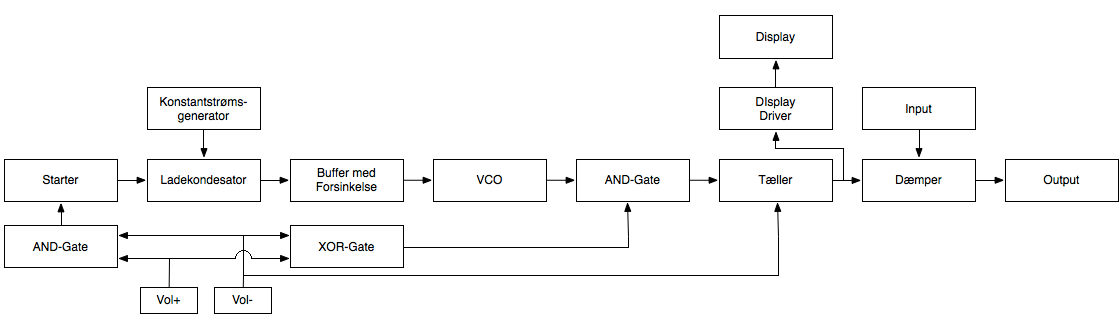
\includegraphics[width=\textwidth]{teknisk/volumenkontrol/blokdiagram.png}
\caption{Blokdiagram over volumenkontrollen}
\label{fig:volumenkontrol_opbygning}
\end{figure}

\begin{figure}[h]
\centering
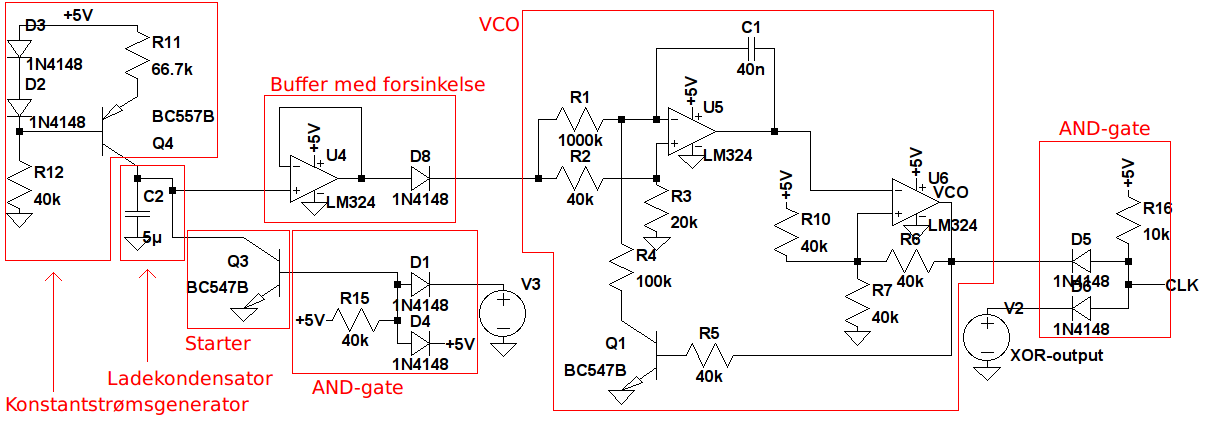
\includegraphics[width=\textwidth]{teknisk/volumenkontrol/diagram.png}
\caption{Diagram over volumenkontrollen}
\label{fig:volumenkontrol_diagram}
\end{figure}

\subsection{Konstantstrømsgenerator}
\label{volumenkontrol-simulering-konstantstroemsgenerator}

Konstantstrømsgeneratorens opgave er at levere en konstant strøm, denne strøm bruges til at oplade en kondensator (ladekondensatoren). Når en kondensator lades med en konstant strøm, vil spændingen over den stige lineært, dette fremgår også af ligning \ref{equ:konstantstroemsgenerator1}.

\begin{equation}
\label{equ:konstantstroemsgenerator1}
V = \frac{I \cdot t}{C}
\end{equation}

Konstantstrømsgeneratoren er designet med udgangs på at der vil være et spændingsfald på 0,5 V over $D_2$, $D_3$, $R_{11}$ og $Q_{4_{BE}}$. I databladet for 1N4148 fremgår det at den vil have en $V_D$ spændingen på 0,5 V ved en $I_F$ strøm på 0,1 mA. Strømmen igennem dioderne er givet ved den strøm, der vil løbe igennem det der kommer efter dem, i dette tilfælde modstanden $R_{12}$. $R_{12}$ er således givet ved ligning \ref{equ:konstantstroemsgenerator2}.

\begin{equation}
\label{equ:konstantstroemsgenerator2}
R_{12} = \frac{V_{CC} - 2 \cdot V_D}{I_F} = \mathrm{\frac{5~V - 2 \cdot 0,5~V}{0,1~mA} = 40~k\ohm}
\end{equation}

Da der nu ligger en konstant spænding over alle dioderne, kan man se dioden i transistoren som siddende parallelt, med det samme spændingsfald som $D_2$. Dette giver at der findes det samme, konstante, spændingsfald over $D_3$ og $R_{11}$, hvilket giver en konstant strøm gennem $R_{11}$.
Den kondensator som konstantstrømsgeneratoren kaldes ladekondensatoren, denne har en kapacitet på 5 $\mu$F og den ønskede oplade tid er 3 s. Kondensatoren oplades fra 0 V til $V_{CC} - V_D$ = 4,5 V, hvor $V_D$ er spændingen over én diode. Udfra disse to ting kan den konstante strøm, $I_{const}$, nu beregnes, se ligning \ref{equ:konstantstroemsgenerator3}.

\begin{equation}
\label{equ:konstantstroemsgenerator3}
V_{CC} - V_D = \frac{I_{const} \cdot t}{C_2} \Rightarrow \mathrm{4,5~V} = \frac{I_{const} \cdot 3~\mathrm{s}}{5~\mu \mathrm{F}} \Rightarrow I_{const} = \mathrm{7,5~\mu A}
\end{equation}

Spændingen over $R_{11}$ er, som tidligere nævnt, 0,5 V og strømmen igennem den er $I_{const}$, der kan Ohms lov bruges til at beregne modstanden, se ligning \ref{equ:konstantstroemsgenerator4}.

\begin{equation}
\label{equ:konstantstroemsgenerator4}
V_D = R_{11} \cdot I_{const} \Rightarrow \mathrm{0,5~V} = R_{11} \cdot \mathrm{7,5~\mu A} \Rightarrow R_{11} = \mathrm{66,7~k\ohm}
\end{equation}

\subsection{Starter}
\label{volumenkontrol-simulering-starter}

Starterens opgave er at holde spændingen over ladekondensatoren på 0 V, når der ikke trykkes på en af volumenknapperne. Dette gøres ved at lede al den strøm som konstantstrømsgeneratoren leverer til stel. Så snart der trykkes på en af volumenknapperne, vil basis på transistoren blive trukket lav, hvilket vil afbryde collector-emitter strømmen. Dette gøres for at sikre at ladekondensatoren er klar til at starte opladningen med det samme.
\subsection{Buffer med forsinkelse}
\label{volumenkontrol-simulering-buffer}

Bufferen sikrer at ladekondensatoren bliver lineært opladet, dette gøres ved ikke at belaste konstantstrømsgeneratoren eller ladekondensatoren. Forsinkelsen laves ved hjælp af en diode. Dioden forsinker signalet ved blot at have et spændingsfald over den, det betyder at spændingen først skal vokse op til minimum en diodespænding, før der kommer en kontrolspænding til VCO'en. Forsinkningen er derfor direkte afhængig af diodespændingen. Dette betyder, at der for at kunne indstille på forsinkelsesperioden skal indsættes en anden diode, med en anden $V_{D}$; eksempelvis en eller flere germaniumsdioder.
